%%
%% Copyright 2007, 2008, 2009 Elsevier Ltd
%%
%% This file is part of the 'Elsarticle Bundle'.
%% ---------------------------------------------
%%
%% It may be distributed under the conditions of the LaTeX Project Public
%% License, either version 1.2 of this license or (at your option) any
%% later version.  The latest version of this license is in
%%    http://www.latex-project.org/lppl.txt
%% and version 1.2 or later is part of all distributions of LaTeX
%% version 1999/12/01 or later.
%%
%% The list of all files belonging to the 'Elsarticle Bundle' is
%% given in the file `manifest.txt'.
%%

%% Template article for Elsevier's document class `elsarticle'
%% with numbered style bibliographic references
%% SP 2008/03/01
%%
%%
%%
%% $Id: elsarticle-template-num.tex 4 2009-10-24 08:22:58Z rishi $
%%
%%
%%\documentclass[preprint,12pt,3p]{elsarticle}

%% Use the option review to obtain double line spacing
\documentclass[preprint,review,12pt]{cs262}

%% Use the options 1p,twocolumn; 3p; 3p,twocolumn; 5p; or 5p,twocolumn
%% for a journal layout:
%% \documentclass[final,1p,times]{elsarticle}
%% \documentclass[final,1p,times,twocolumn]{elsarticle}
%% \documentclass[final,3p,times]{elsarticle}
%% \documentclass[final,3p,times,twocolumn]{elsarticle}
%% \documentclass[final,5p,times]{elsarticle}
%% \documentclass[final,5p,times,twocolumn]{elsarticle}

%% if you use PostScript figures in your article
%% use the graphics package for simple commands
%% \usepackage{graphics}
%% or use the graphicx package for more complicated commands
%% \usepackage{graphicx}
%% or use the epsfig package if you prefer to use the old commands
%% \usepackage{epsfig}

%% The amssymb package provides various useful mathematical symbols
\usepackage{amssymb}
\usepackage{color}

%% The amsthm package provides extended theorem environments
%% \usepackage{amsthm}

%% The lineno packages adds line numbers. Start line numbering with
%% \begin{linenumbers}, end it with \end{linenumbers}. Or switch it on
%% for the whole article with \linenumbers after \end{frontmatter}.
%% \usepackage{lineno}

%% natbib.sty is loaded by default. However, natbib options can be
%% provided with \biboptions{...} command. Following options are
%% valid:

%%   round  -  round parentheses are used (default)
%%   square -  square brackets are used   [option]
%%   curly  -  curly braces are used      {option}
%%   angle  -  angle brackets are used    <option>
%%   semicolon  -  multiple citations separated by semi-colon
%%   colon  - same as semicolon, an earlier confusion
%%   comma  -  separated by comma
%%   numbers-  selects numerical citations
%%   super  -  numerical citations as superscripts
%%   sort   -  sorts multiple citations according to order in ref. list
%%   sort&compress   -  like sort, but also compresses numerical citations
%%   compress - compresses without sorting
%%
%% \biboptions{comma,round}

% \biboptions{}

\newcommand{\note}[3]{{\color{#2}[#1: #3]}}
%\newcommand{\note}[3]{}%remove comments
\newcommand{\SERENA}[1]{\note{SERENA}{red}{#1}}
\newcommand{\MICHELLE}[1]{\note{MICHELLE}{blue}{#1}}


\journal{CS262: Distributed Systems}

\begin{document}

\begin{frontmatter}

\title{\texttt{ConnectedHearts}: \\ A Distributed System for Viewing the Human Heartbeat}

\author[label1, label0]{Serena Booth}
\address[label1]{sbooth@college.harvard.edu}


\author[label2, label0]{Michelle Cone}
\address[label2]{mcone@college.harvard.edu}

\fntext[label0]{We, Serena Booth and Michelle Cone, affirm our awareness of the standards of the Harvard College Honor Code.}

\begin{abstract}
We present a physical distributed system for viewing the human heartbeat. We modified a medicine cabinet by embedding 13 light bulbs around the frame, as well as by replacing the cabinet's glass with one-way mirror. When a person stands in front of the mirror, a webcam hidden behind the mirror measures their pulse. The 13 bulbs, each a virtual machine, run Bully leader election. First the leader starts pulsating with the captured pulse, and then instructs neighboring virtual machines to pulsate as well. Finally, we ensure the synchronization of the bulbs through a distributed gossip algorithm.
\end{abstract}

% \begin{keyword}
% %% keywords here, in the form: keyword \sep keyword
% example \sep \LaTeX \sep template
% %% MSC codes here, in the form: \MSC code \sep code
% %% or \MSC[2008] code \sep code (2000 is the default)
% \end{keyword}

\end{frontmatter}

%%
%% Start line numbering here if you want
%%
% \linenumbers


%% main text
\section{Introduction}
\label{sec1}

\texttt{ConnectedHearts} straddles the boundary between art and computer science. The piece is inspired by an exhibit shown around the world in modern art museums, but our re-implementation emphasizes distributed computing, as \texttt{ConnectedHearts} is a physical representation of a distributed system. We modify a retro medicine cabinet to hold 13 light bulbs around its frame. While in an ideal world each light bulb would be powered by its own microprocessor, we simulate this interaction instead by each light bulb representing a virtual machine as a process in effort to reduce expenditure. These light bulbs attempt to self-synchronize while displaying the human heartbeat. 

In this paper, we discuss the components and construction of  \texttt{Connected Hearts}, the architecture and algorithms powering the software, as well as analysis of our system. 

\subsection{Artistic Inspiration}

This piece is inspired by Rafael Lorzeno-Hemmer's ``Pulse Room,''\cite{pulse} an artistic piece in which an entire room is outfitted with light bulbs. A physical heartbeat monitor is present in the room. A user approaches this monitor and grabs onto it. As soon as the conductance of the skin is felt, all light bulbs in the room turn off. Within a few seconds, the heartbeat monitor detects a pulse. With this, a single bulb directly above the user begins to pulsate with their heartbeat. This message is then spread to neighboring bulbs, as well as bouncing off of the walls; with this message-passing, the room becomes full of chaos. After a further few minutes, the bulbs synchronize, leaving the entire room pulsating with the heartbeat. We note that this system uses a single address-space to achieve this effect. 


\section{Components \& Construction}

\noindent We construct the piece from the following materials:
\begin{itemize} 
\item 2 $\times$ Ubiquiti mPower Strips: 8-outlet power strips running Linux
\item Network switch and ethernet cables
\item 13 $\times$ filament bulbs and bulb holders
\item Vintage Medicine Cabinet, one-way glass
\item Raspberry Pi
\item Raspberry PiCamera
\end{itemize} 

The end product looks to be a medicine cabinet with 13 light bulbs around its mirror; the majority of the components---the cables, the Raspberry Pi, etc.---are hidden from view, inside the cabinet. 

\section{System Design}

Our code is written in Python and makes extensive use of the multiprocessing library. 

\SERENA{TO DO: Explain process layout + relationships} 

\subsection{Inter-bulb Communication}

\section{Architecture \& Algorithms}

\subsection{Pulse Detection} 

When a face is visible to a camera hidden behind the one-way glass of the medicine cabinet, we detect the pulse of the viewer. 

\subsection{Bully: Leader Election}

\SERENA{TO DO: Write about Bully}

We demonstrate this leader election mechanism in Figure \ref{fig:bully}. 
\begin{figure}
  \centering
  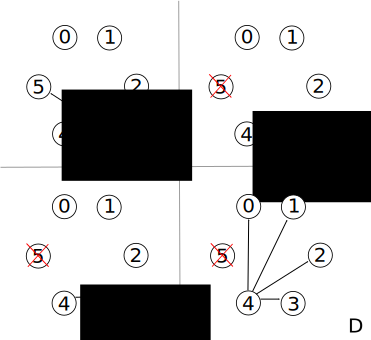
\includegraphics[width=0.7\textwidth]{figures/bully}
  \caption{In the above graphic, we demonstrate the bully algorithm for determining a leader. In subimage A, node 3 attempts to confirm that the known leader, node 5, is still alive. In sumbimage B, node 5 does not respond to node 3 for a set period of time---a time set by node 3. Hence node 3 initiates an election by contacting all nodes with a higher id than itself. In subimage C, node 4 responds to node 3's request to initiate an election by confirming it remains alive. Finally, in subimage D, node 4 broadcasts a message to all nodes to inform them of its leader status. 
 \label{fig:bully}}
\end{figure}

\subsection{Realtime Synchronization via Gossip}
\SERENA{TO DO: Write about synchronization}
\subsubsection{Physical Layout}

\begin{figure}[h]
  \centering
  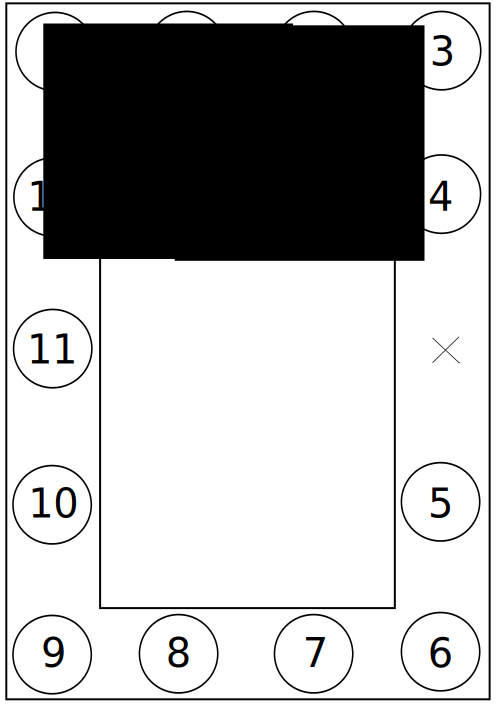
\includegraphics[width=0.3\textwidth]{figures/system_layout}
  \caption{The system layout. While each bulb is assigned a 64-bit UUID during the program, each bulb also has an id, shown above, ranging from $0-12$, which allows the system to consistently converge toward the leader bulb's rate of pulsation during the synchronization routine. 
 \label{fig:layout}}
\end{figure}

The physical layout of our system is predetermined, as shown in Figure \ref{fig:layout}. Each bulb is assigned a fixed, position-based id as well as a generated UUID. Because of this fixed layout, we are able to personalize gossip for synchronization in order to ascribe neighboring processes with scores of \emph{trustworthiness}. As the leader bulb initiates the heartbeat pulsation, the leader is the single most trustworthy bulb. This has implications for all other bulbs, however: as bulbs increase in distance from the leader, a known measure based on the system's fixed layout, their trustworthiness decreases. Thus when a bulb is receiving contradictory gossip from its two neighboring bulbs, it prioritizes the message which was sent by the bulb closer to the leader.  

\section{Synchronization Testing \& Analysis}

In order to analyze the success of our synchronization via gossip, we implement a simple computer vision system. The steps of analysis are as follows: 

\begin{enumerate} 
\item We capture footage at a high-frame rate. 

- 120 fps; however, we note that this frame rate is slower than the processing rate of the human eye. 

\item With GUI, present user with first frame of the captured footage. 

- User selects 13 pixels corresponding to bulb filaments. 

\item Brightness timeseries computed. 

- The brightness of these pixels are averaged for every frame in the video, and ultimately we produce a timeseries, which we graph in comparison to idealized data. A demonstration of this result is shown in Figure \ref{fig:res}. 
\end{enumerate}

\begin{figure}[h]
  \centering
  \includegraphics[width=\textwidth]{figures/results}
  \caption{We demonstrate the synchronization of our system as a function of time, as compared with an ideal synchronization system. The green timeseries corresponds to the physical system while the blue timeseries corresponds to an idealized system. 
 \label{fig:res}}
\end{figure}

\section{Personal Learning} 


\begin{enumerate}
\item Debugging a distributed system is hard. 
\end{enumerate}

\section{Conclusion}



%% The Appendices part is started with the command \appendix;
%% appendix sections are then done as normal sections

%% References
%%
%% Following citation commands can be used in the body text:
%% Usage of \cite is as follows:
%%   \cite{key}         ==>>  [#]
%%   \cite[chap. 2]{key} ==>> [#, chap. 2]
%%

%% References with bibTeX database:

\bibliographystyle{elsarticle-num}
% \bibliographystyle{elsarticle-harv}
% \bibliographystyle{elsarticle-num-names}
% \bibliographystyle{model1a-num-names}
% \bibliographystyle{model1b-num-names}
% \bibliographystyle{model1c-num-names}
% \bibliographystyle{model1-num-names}
% \bibliographystyle{model2-names}
% \bibliographystyle{model3a-num-names}
% \bibliographystyle{model3-num-names}
% \bibliographystyle{model4-names}
% \bibliographystyle{model5-names}
% \bibliographystyle{model6-num-names}

\bibliography{sample}


\end{document}

%%
%% End of file `elsarticle-template-num.tex'.
